\documentclass[compress]{beamer}
\usepackage{ifthen,verbatim}

\title{Updates in Muon Alignment}
\author{Jim Pivarski, Karoly Banicz, Alexey Kamenev, Alexei Safonov}
\institute{Texas A\&M University}
\date{ 9 August, 2007}

\newcommand{\isnote}{}
\xdefinecolor{lightyellow}{rgb}{1.,1.,0.25}
\xdefinecolor{darkblue}{rgb}{0.1,0.1,0.7}

%% Uncomment this to get annotations
%% \def\notes{\addtocounter{page}{-1}
%%            \renewcommand{\isnote}{*}
%% 	   \beamertemplateshadingbackground{lightyellow}{white}
%%            \begin{frame}
%%            \frametitle{Notes for the previous page (page \insertpagenumber)}
%%            \itemize}
%% \def\endnotes{\enditemize
%% 	      \end{frame}
%%               \beamertemplateshadingbackground{white}{white}
%%               \renewcommand{\isnote}{}}

%% Uncomment this to not get annotations
\def\notes{\comment}
\def\endnotes{\endcomment}

\setbeamertemplate{navigation symbols}{}
\setbeamertemplate{headline}{\includegraphics[height=1 cm]{../cmslogo} \hspace{0.1 cm} \includegraphics[height=1 cm]{../tamulogo} \hfill
\begin{minipage}{5.5 cm}
\vspace{-0.75 cm} \small
\begin{center}
\ifthenelse{\equal{\insertpagenumber}{1}}{}{\textcolor{blue}{\insertsection}}
\end{center}
\end{minipage} \hfill
\begin{minipage}{4.5 cm}
\vspace{-0.75 cm} \small
\begin{flushright}
\ifthenelse{\equal{\insertpagenumber}{1}}{}{Jim Pivarski \hspace{0.5 cm} \insertpagenumber\isnote/\pageref{numpages}}
\end{flushright}
\end{minipage}\mbox{\hspace{0.2 cm}}}

\begin{document}
\frame{\titlepage}

\begin{notes}
\item This is the annotated version of my talk.
\item If you want the version that I am presenting, download the one
labeled ``slides'' on Indico (or just ignore these yellow pages).
\item The annotated version is provided for extra detail and a written
record of comments that I intend to make orally.
\item Yellow notes refer to the content on the {\it previous} page.
\item All other slides are identical for the two versions.
\end{notes}

\section*{Overview}

\begin{frame}
\frametitle{Since July\ldots}
\begin{itemize}\setlength{\itemsep}{0.75 cm}
\item Alignment procedure ported to 1\_5\_X/1\_6\_X, fully documented
\item Alignment projects split by task, not by detector

\vspace{0.25 cm}
\begin{itemize}\setlength{\itemsep}{0.5 cm}
\item Karoly: investigating beam halo MC for beam halo alignment
\item Alexey: investigating cosmics MC for MTCC alignment \\ (all stations, not only ME1/1)
\item Jim: systematics studies for disk-by-disk (and wheel-by-wheel) alignment, preparing for CSA07
\end{itemize}

\item Using the same software; meeting weekly
\end{itemize}
\end{frame}

\section*{Karoly: beam halo alignment (CSC)}

\begin{frame}
\begin{itemize}\setlength{\itemsep}{0.4 cm}
\item One-beam generator-level study: 2000 Hz?
\begin{center}
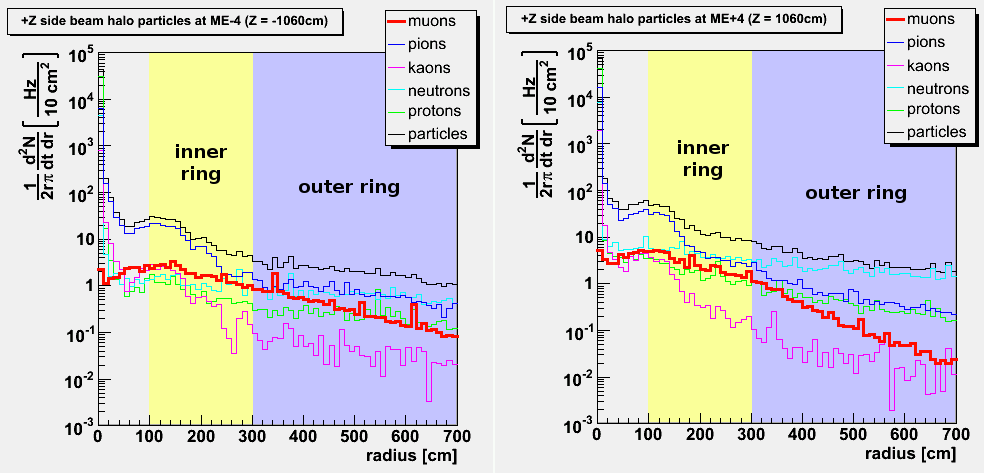
\includegraphics[width=\linewidth]{beam_halo_profiles.png}
\end{center}

\item Generated 10,000 events, found 1,600 standalone muons (CosmicMuonProducer), some events have 2 muons

\item Tested full alignment path!
\end{itemize}
\end{frame}

\section*{Alexey: cosmic ray/MTCC (CSC)}

\begin{frame}
\begin{itemize}\setlength{\itemsep}{1 cm}
\item Just started, working through the documentation\ldots
\item Will need cosmic ray MC, re-reconstructed MTCC
\end{itemize}
\end{frame}

\section*{Jim: disk-by-disk/wheel-by-wheel}

\begin{frame}
\begin{itemize}\setlength{\itemsep}{0.75 cm}
  \item Pessimistic internal misalignments (chambers and layers)
    \begin{itemize}\setlength{\itemsep}{0.25 cm}
    \item CSC Layers $\Delta x = 191$ $\mu$m, $\Delta y = 335$ $\mu$m, $\Delta \phi_z = 40$ $\mu$rad
    \item All Chambers $\Delta x = \Delta y = \Delta z = 3$ mm, \\ \textcolor{white}{All Chambers} $\Delta \phi_x = \Delta \phi_y = \Delta \phi_z = 1$ mrad
    \item Disks/wheels $\Delta x = \Delta y = \Delta z = 1$ cm, \\ \textcolor{white}{Disks/wheels} $\Delta \phi_x = \Delta \phi_y = \Delta \phi_z = 1$ mrad
    \item Tracker 10 pb$^{-1}$ scenario
    \end{itemize}

  \item Align muon system to tracker with globalMuons: $x$, $y$, $\phi_z$
\begin{itemize}
  \item Check dependence on tracker alignment
\end{itemize}

  \item Nominally 2000 $Z\to\mu\mu$ (0.36 pb$^{-1}$)
\begin{itemize}
  \item Check dependence on statistics
\end{itemize}
\end{itemize}
\end{frame}

\begin{frame}
\begin{center}
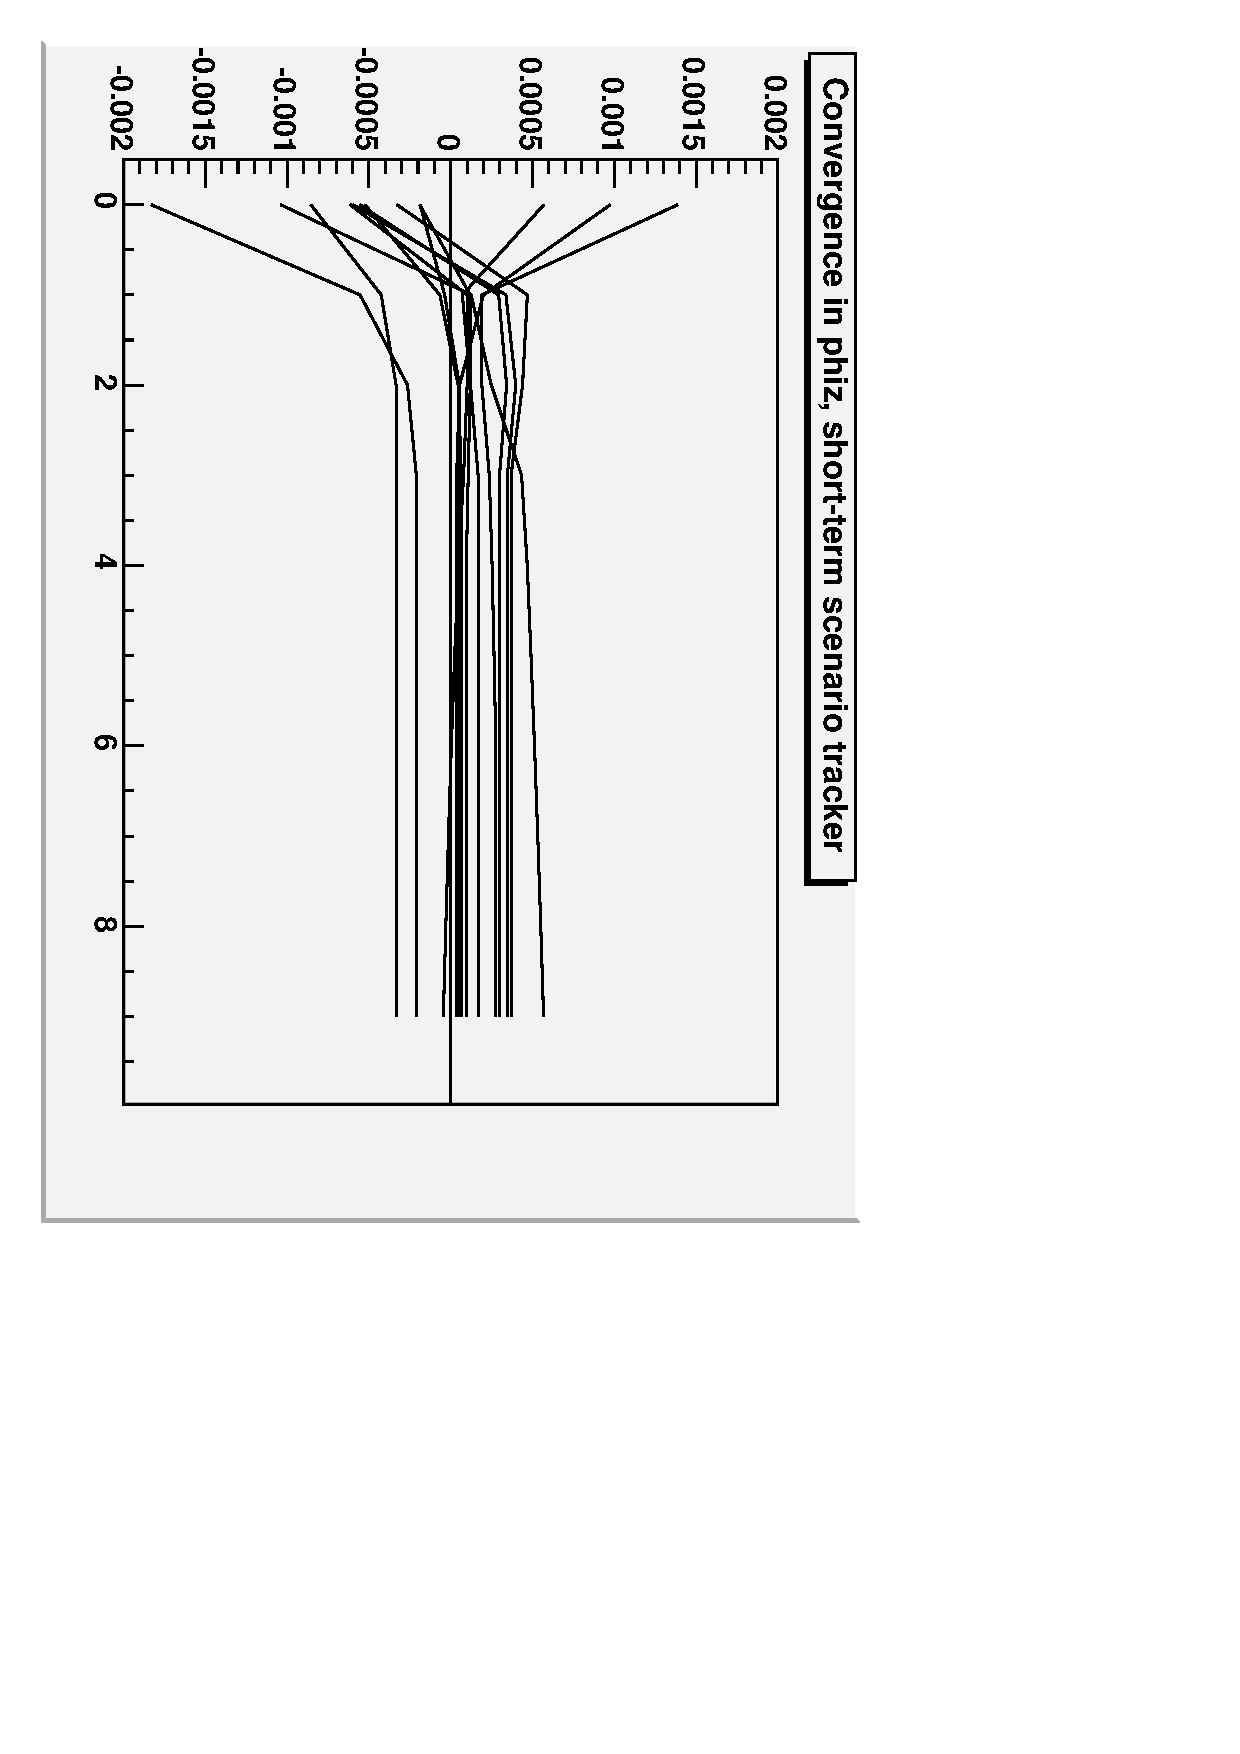
\includegraphics[height=0.5\linewidth, angle=90]{phiz_conv_nominal.pdf} 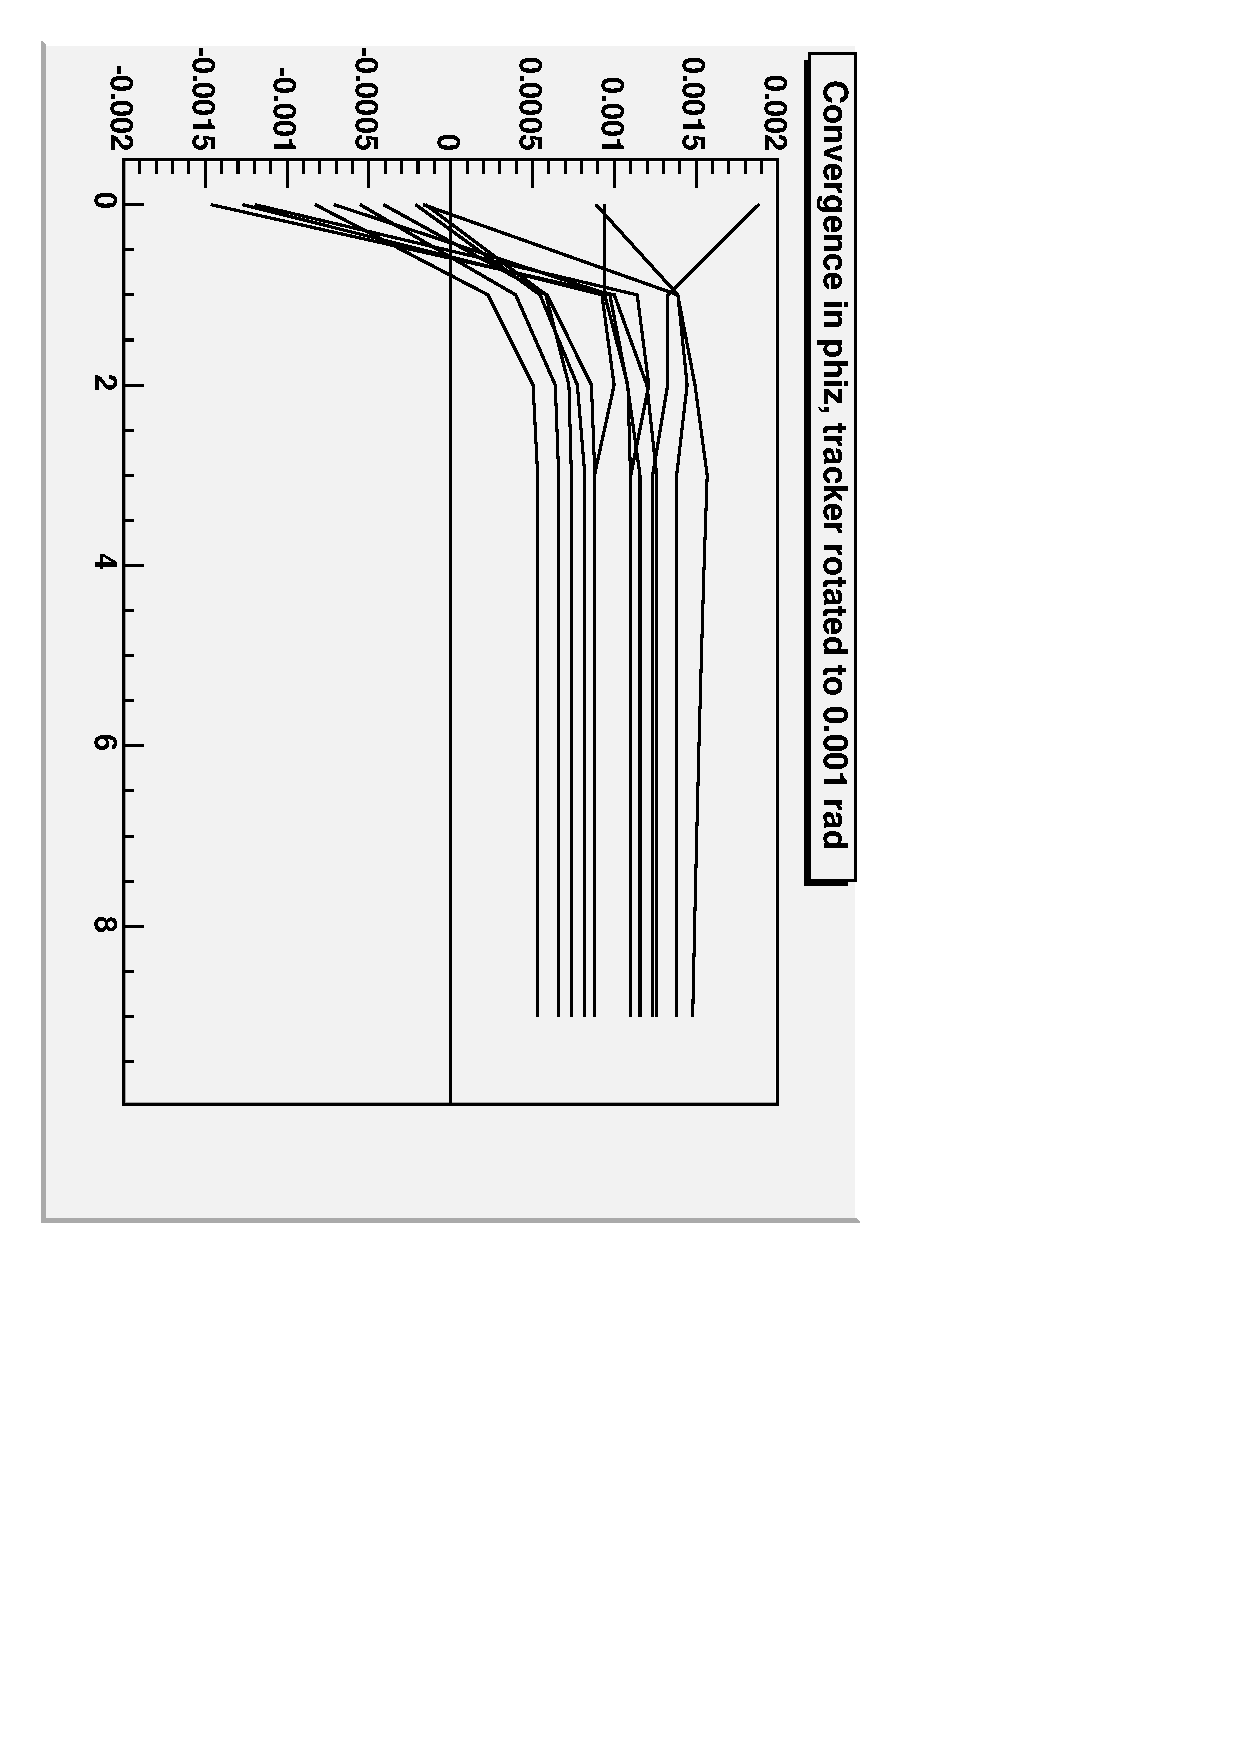
\includegraphics[height=0.5\linewidth, angle=90]{phiz_conv_barrel_roll.pdf}
\end{center}

\begin{itemize}
\item 0.3 mrad resolution in $\phi_z$, 800 $\mu$m in $x$, $y$
\item Large numbers of tracks are unnecessary: reaches final precision with a few hundred muons
\item Sensitive to tracker alignment: rotate tracker by 1 mrad (sanity check)
\end{itemize}
\end{frame}

\begin{frame}
\frametitle{Sensitivity to tracker misalignment}
{\small \mbox{ } \hfill black: with internal misalignments \hfill \textcolor{red}{red: ideal chambers, layers} \hfill \mbox{ }}
\begin{center}
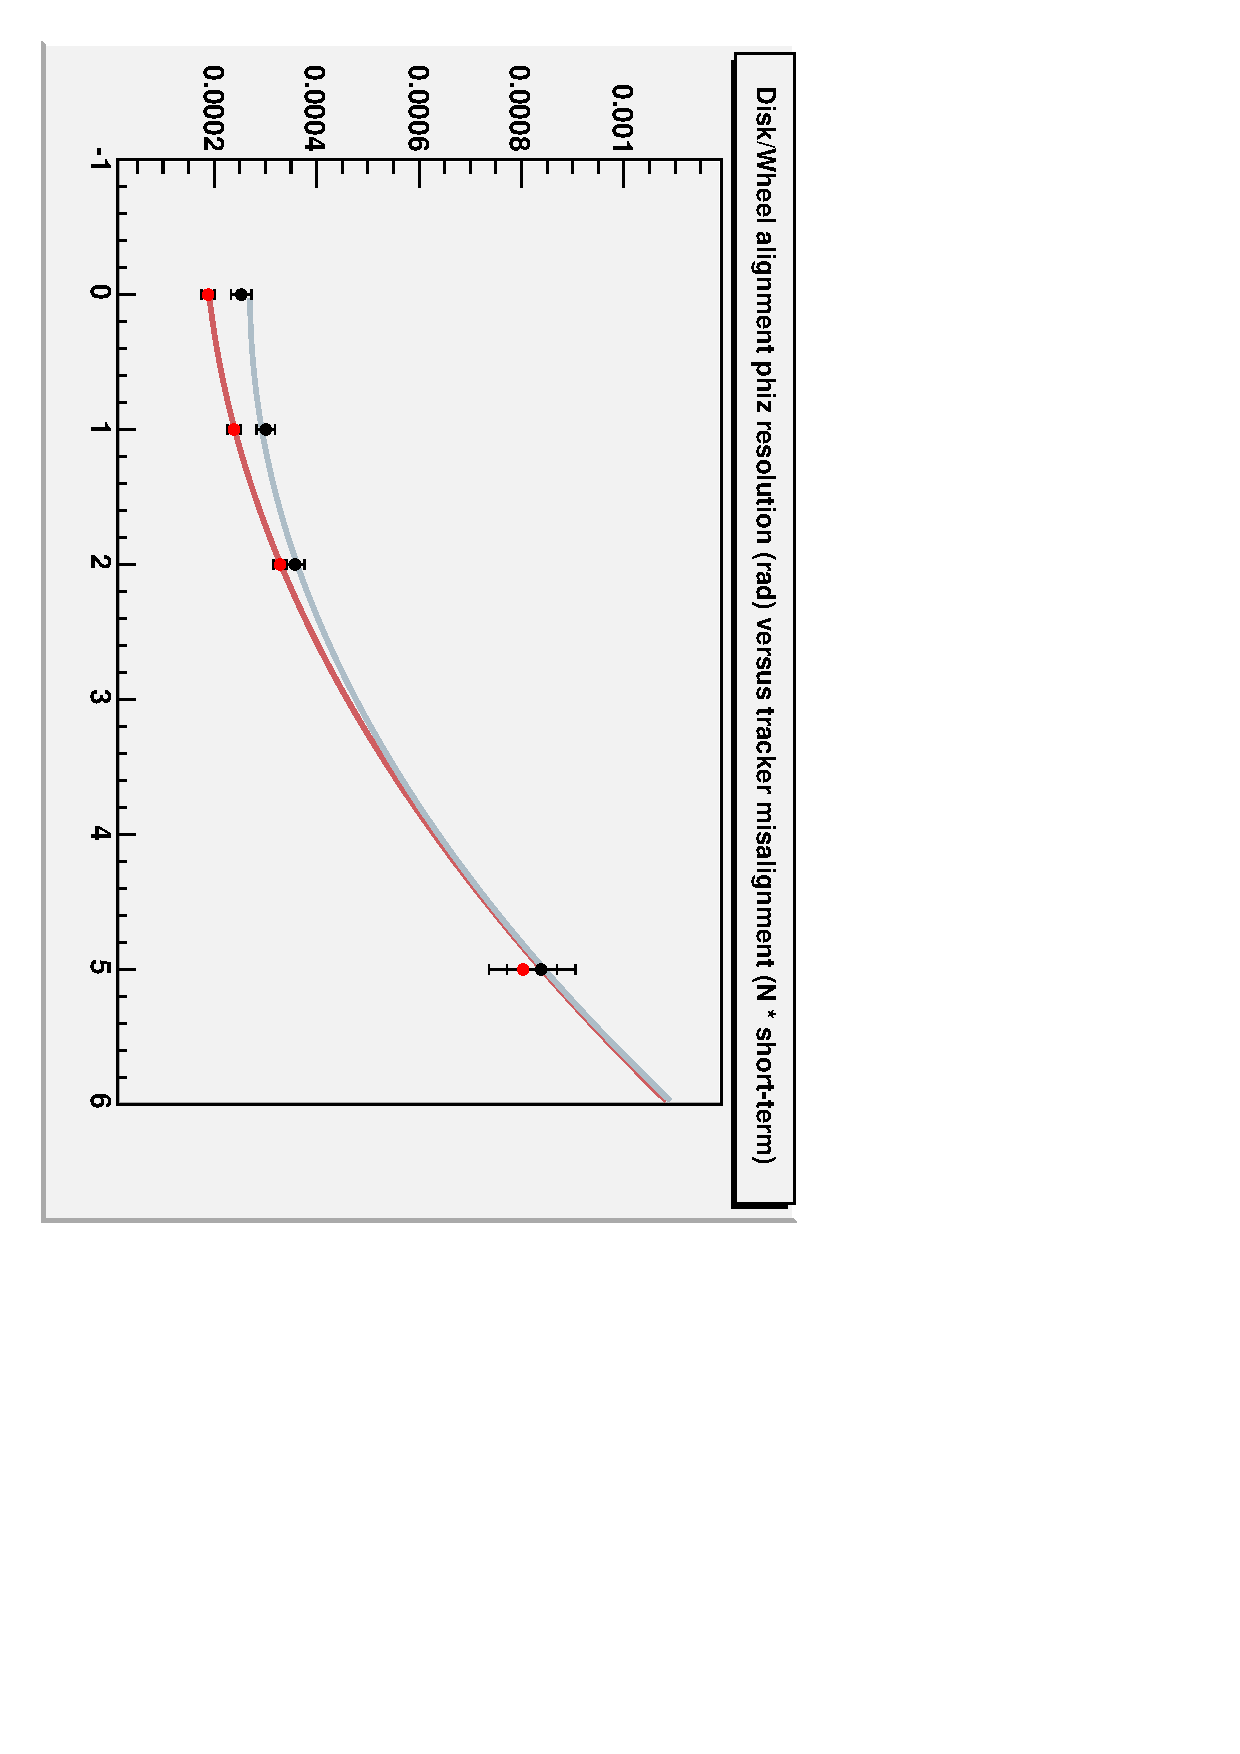
\includegraphics[height=0.7\linewidth, angle=90]{vstracker2.pdf}
\end{center}

\begin{itemize}
\item 13 disks+wheels is not enough to measure precision: 10 trials
\item Tracker can be 2--3 times worse than short-term scenario
\end{itemize}
\end{frame}

\begin{frame}
\frametitle{Varying Alignment Parameter Errors versus iteration}
\begin{center}
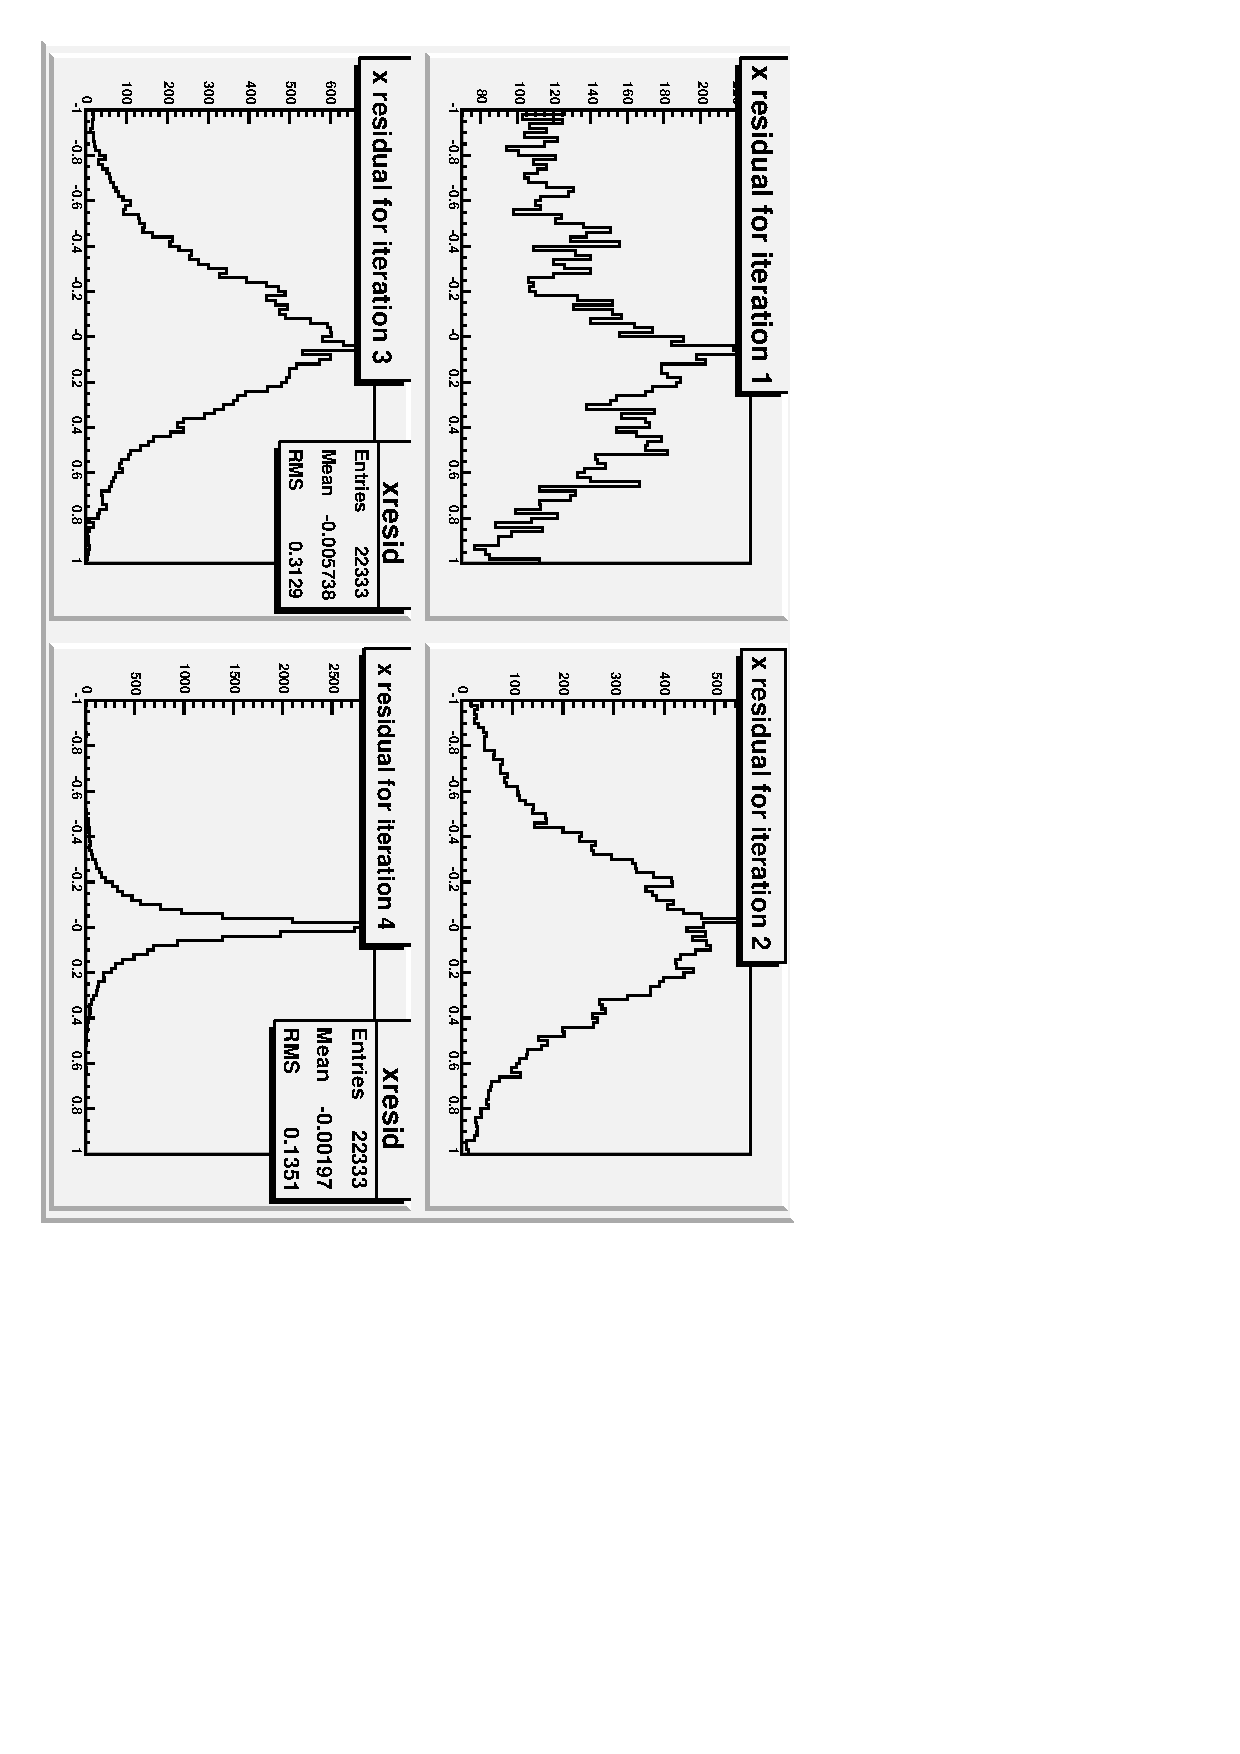
\includegraphics[height=0.8\linewidth, angle=90]{residuals_by_iteration.pdf}
\end{center}
\begin{itemize}
\item Iterations 1--3: APEs $\gg$ intrinsic errors
\item Iterations 4--10: APEs $\ll$ intrinsic errors; alignments stable
\end{itemize}
\end{frame}

\section*{Preparation for CSA07}

\begin{frame}
\begin{itemize}\setlength{\itemsep}{0.65 cm}
\item CAF alignment farm is ready and working
\item Discovered that RPC hits bias alignments toward ideal geometry:
making sure they are excluded from alignment fits
\item Pre-CSA test with 1 million $Z\to\mu\mu$, 1 million $W\to\mu\nu$

\vspace{0.1 cm}
\begin{itemize}\setlength{\itemsep}{0.25 cm}
\item Ideal, 10 pb$^{-1}$ miscal/misalign, 100 pb$^{-1}$ miscal/misalign
\item Can we align with miscalibrations?
\end{itemize}
\item Pre-pre-CSA test with 75,000 single-muons

\vspace{0.1 cm}
\begin{itemize}\setlength{\itemsep}{0.25 cm}
\item Chamber-by-chamber dependence on tracker misalignment
\item Study momentum dependence (10 GeV and 100 GeV)
\end{itemize}
\end{itemize}
\end{frame}

\section*{Summary}

\begin{frame}
\begin{itemize}\setlength{\itemsep}{0.75 cm}
\item Beam-halo alignments: we have a simulation, a small dataset, and are beginning alignment studies
\item Cosmic ray alignments: just beginning--- we'll need MC, re-reconstructed MTCC
\item Collision-data alignments: finished tracker-dependence studies
for disk-by-disk, moving on to chamber-by-chamber studies
\end{itemize}
\label{numpages}
\end{frame}

\end{document}
